\documentclass[english]{lni}
\usepackage{latin1}

%\usepackage{times}
\usepackage{ifpdf}
%\usepackage{a4wide}
%\usepackage{pdfsync}

\ifpdf 
  \usepackage[pdftex]{graphicx} 
\else 
  \usepackage{graphicx} 
\fi

\usepackage{xspace} 
%\usepackage{tabularx} 
%\usepackage{epsfig}
%\usepackage{amsmath} 
%\usepackage{amsfonts} 
%\usepackage{amssymb}
%\usepackage{eucal} 
%\usepackage{stmaryrd} 
\usepackage{float}
\usepackage{listings} 

% @(#)$Id: jml-listings.tex,v 1.6 2007/06/25 22:37:23 leavens Exp $
%
% Copyright (C) 2006 Iowa State University
%
% This file is part of JML
%
% JML is free software; you can redistribute it and/or modify
% it under the terms of the GNU General Public License as published by
% the Free Software Foundation; either version 2, or (at your option)
% any later version.
%
% JML is distributed in the hope that it will be useful,
% but WITHOUT ANY WARRANTY; without even the implied warranty of
% MERCHANTABILITY or FITNESS FOR A PARTICULAR PURPOSE.  See the
% GNU General Public License for more details.
%
% You should have received a copy of the GNU General Public License
% along with JML; see the file COPYING.  If not, write to
% the Free Software Foundation, 675 Mass Ave, Cambridge, MA 02139, USA.
%
% A JML listings environment.
%
% AUTHOR: Gary T. Leavens
%
% requires listings i.e., do \usepackage{listings} first
%
% This file is set up to be used via % @(#)$Id: jml-listings.tex,v 1.6 2007/06/25 22:37:23 leavens Exp $
%
% Copyright (C) 2006 Iowa State University
%
% This file is part of JML
%
% JML is free software; you can redistribute it and/or modify
% it under the terms of the GNU General Public License as published by
% the Free Software Foundation; either version 2, or (at your option)
% any later version.
%
% JML is distributed in the hope that it will be useful,
% but WITHOUT ANY WARRANTY; without even the implied warranty of
% MERCHANTABILITY or FITNESS FOR A PARTICULAR PURPOSE.  See the
% GNU General Public License for more details.
%
% You should have received a copy of the GNU General Public License
% along with JML; see the file COPYING.  If not, write to
% the Free Software Foundation, 675 Mass Ave, Cambridge, MA 02139, USA.
%
% A JML listings environment.
%
% AUTHOR: Gary T. Leavens
%
% requires listings i.e., do \usepackage{listings} first
%
% This file is set up to be used via % @(#)$Id: jml-listings.tex,v 1.6 2007/06/25 22:37:23 leavens Exp $
%
% Copyright (C) 2006 Iowa State University
%
% This file is part of JML
%
% JML is free software; you can redistribute it and/or modify
% it under the terms of the GNU General Public License as published by
% the Free Software Foundation; either version 2, or (at your option)
% any later version.
%
% JML is distributed in the hope that it will be useful,
% but WITHOUT ANY WARRANTY; without even the implied warranty of
% MERCHANTABILITY or FITNESS FOR A PARTICULAR PURPOSE.  See the
% GNU General Public License for more details.
%
% You should have received a copy of the GNU General Public License
% along with JML; see the file COPYING.  If not, write to
% the Free Software Foundation, 675 Mass Ave, Cambridge, MA 02139, USA.
%
% A JML listings environment.
%
% AUTHOR: Gary T. Leavens
%
% requires listings i.e., do \usepackage{listings} first
%
% This file is set up to be used via \input{jml-listings}.
% If you want, you could make a version that is a style file,
% but then change \lstdefinelanguage to \lst@definelanguage below.
%
\lstdefinelanguage[JML]{Java}[]{Java}%
       {% C++ style comments have to start with a blank!
        comment=[l]{//\ },
        % And C-style comments must also start with a blank or star!
        morecomment=[s]{/*\ }{*/},        
        morecomment=[s]{/**}{*/},
        % sensitive=true, % inherited
        % Add JML keywords as level 1 keywords, so can typeset differently
        classoffset=1,
        % And here are all the wonderful JML keywords
        morekeywords={abrupt_behavior,abrupt_behaviour,
         accessible,accessible_redundantly,also,assert,assert_redundantly,
         assignable,assignable_redundantly,assume,assume_redundantly,
         axiom,behavior,behaviour,breaks,breaks_redundantly,
         callable,callable_redundantly,captures,captures_redundantly,
         choose,choose_if,code,code_bigint_math,code_java_math,
         code_safe_math,constraint,constraint_redundantly,constructor,
         continues,continues_redundantly,decreases,decreases_redundantly,
         decreasing,decreasing_redundantly,diverges,diverges_redundantly,
         duration,duration_redundantly,ensures,ensures_redundantly,
         example,exceptional_behavior,exceptional_behaviour,
         exceptional_example,exsures,exsures_redundantly,extract,field,
         forall,for_example,ghost,helper,hence_by,hence_by_redundantly,
         implies_that,in,in_redundantly,initializer,initially,instance,
         invariant,invariant_redundantly,loop_invariant,
         loop_invariant_redundantly,maintaining,maintaining_redundantly,
         maps,maps_redundantly,measured_by,measured_by_redundantly,method,
         model,model_program,modifiable,modifiable_redundantly,modifies,
         modifies_redundantly,monitored,monitors_for,non_null,
         normal_behavior,normal_behaviour,normal_example,nowarn,
         nullable,nullable_by_default,old,or,post,post_redundantly,
         pre,pre_redundantly,pure,readable,refine,refines,refining,represents,
         represents_redundantly,requires,requires_redundantly,
         returns,returns_redundantly,set,signals,signals_only,
         signals_only_redundantly,signals_redundantly,spec_bigint_math,
         spec_java_math,spec_protected,spec_public,spec_safe_math,
         static_initializer,uninitialized,unreachable,weakly,
         when,when_redundantly,working_space,working_space_redundantly,
         writable
        },
        % keywords from the universe type system
        morekeywords={rep,peer,readonly},
        % typeset everything that starts with a backslash as a keyword
        % BUG: this doesn't allow typesetting these keywords differently
        keywordsprefix=\\,
        otherkeywords={<:,<-,->,..,<==,==>,<==>,<=!=>},
        classoffset=0 % restore default class for keywords
}
.
% If you want, you could make a version that is a style file,
% but then change \lstdefinelanguage to \lst@definelanguage below.
%
\lstdefinelanguage[JML]{Java}[]{Java}%
       {% C++ style comments have to start with a blank!
        comment=[l]{//\ },
        % And C-style comments must also start with a blank or star!
        morecomment=[s]{/*\ }{*/},        
        morecomment=[s]{/**}{*/},
        % sensitive=true, % inherited
        % Add JML keywords as level 1 keywords, so can typeset differently
        classoffset=1,
        % And here are all the wonderful JML keywords
        morekeywords={abrupt_behavior,abrupt_behaviour,
         accessible,accessible_redundantly,also,assert,assert_redundantly,
         assignable,assignable_redundantly,assume,assume_redundantly,
         axiom,behavior,behaviour,breaks,breaks_redundantly,
         callable,callable_redundantly,captures,captures_redundantly,
         choose,choose_if,code,code_bigint_math,code_java_math,
         code_safe_math,constraint,constraint_redundantly,constructor,
         continues,continues_redundantly,decreases,decreases_redundantly,
         decreasing,decreasing_redundantly,diverges,diverges_redundantly,
         duration,duration_redundantly,ensures,ensures_redundantly,
         example,exceptional_behavior,exceptional_behaviour,
         exceptional_example,exsures,exsures_redundantly,extract,field,
         forall,for_example,ghost,helper,hence_by,hence_by_redundantly,
         implies_that,in,in_redundantly,initializer,initially,instance,
         invariant,invariant_redundantly,loop_invariant,
         loop_invariant_redundantly,maintaining,maintaining_redundantly,
         maps,maps_redundantly,measured_by,measured_by_redundantly,method,
         model,model_program,modifiable,modifiable_redundantly,modifies,
         modifies_redundantly,monitored,monitors_for,non_null,
         normal_behavior,normal_behaviour,normal_example,nowarn,
         nullable,nullable_by_default,old,or,post,post_redundantly,
         pre,pre_redundantly,pure,readable,refine,refines,refining,represents,
         represents_redundantly,requires,requires_redundantly,
         returns,returns_redundantly,set,signals,signals_only,
         signals_only_redundantly,signals_redundantly,spec_bigint_math,
         spec_java_math,spec_protected,spec_public,spec_safe_math,
         static_initializer,uninitialized,unreachable,weakly,
         when,when_redundantly,working_space,working_space_redundantly,
         writable
        },
        % keywords from the universe type system
        morekeywords={rep,peer,readonly},
        % typeset everything that starts with a backslash as a keyword
        % BUG: this doesn't allow typesetting these keywords differently
        keywordsprefix=\\,
        otherkeywords={<:,<-,->,..,<==,==>,<==>,<=!=>},
        classoffset=0 % restore default class for keywords
}
.
% If you want, you could make a version that is a style file,
% but then change \lstdefinelanguage to \lst@definelanguage below.
%
\lstdefinelanguage[JML]{Java}[]{Java}%
       {% C++ style comments have to start with a blank!
        comment=[l]{//\ },
        % And C-style comments must also start with a blank or star!
        morecomment=[s]{/*\ }{*/},        
        morecomment=[s]{/**}{*/},
        % sensitive=true, % inherited
        % Add JML keywords as level 1 keywords, so can typeset differently
        classoffset=1,
        % And here are all the wonderful JML keywords
        morekeywords={abrupt_behavior,abrupt_behaviour,
         accessible,accessible_redundantly,also,assert,assert_redundantly,
         assignable,assignable_redundantly,assume,assume_redundantly,
         axiom,behavior,behaviour,breaks,breaks_redundantly,
         callable,callable_redundantly,captures,captures_redundantly,
         choose,choose_if,code,code_bigint_math,code_java_math,
         code_safe_math,constraint,constraint_redundantly,constructor,
         continues,continues_redundantly,decreases,decreases_redundantly,
         decreasing,decreasing_redundantly,diverges,diverges_redundantly,
         duration,duration_redundantly,ensures,ensures_redundantly,
         example,exceptional_behavior,exceptional_behaviour,
         exceptional_example,exsures,exsures_redundantly,extract,field,
         forall,for_example,ghost,helper,hence_by,hence_by_redundantly,
         implies_that,in,in_redundantly,initializer,initially,instance,
         invariant,invariant_redundantly,loop_invariant,
         loop_invariant_redundantly,maintaining,maintaining_redundantly,
         maps,maps_redundantly,measured_by,measured_by_redundantly,method,
         model,model_program,modifiable,modifiable_redundantly,modifies,
         modifies_redundantly,monitored,monitors_for,non_null,
         normal_behavior,normal_behaviour,normal_example,nowarn,
         nullable,nullable_by_default,old,or,post,post_redundantly,
         pre,pre_redundantly,pure,readable,refine,refines,refining,represents,
         represents_redundantly,requires,requires_redundantly,
         returns,returns_redundantly,set,signals,signals_only,
         signals_only_redundantly,signals_redundantly,spec_bigint_math,
         spec_java_math,spec_protected,spec_public,spec_safe_math,
         static_initializer,uninitialized,unreachable,weakly,
         when,when_redundantly,working_space,working_space_redundantly,
         writable
        },
        % keywords from the universe type system
        morekeywords={rep,peer,readonly},
        % typeset everything that starts with a backslash as a keyword
        % BUG: this doesn't allow typesetting these keywords differently
        keywordsprefix=\\,
        otherkeywords={<:,<-,->,..,<==,==>,<==>,<=!=>},
        classoffset=0 % restore default class for keywords
}

\lstset{language=[JML]Java,xleftmargin=20pt,xrightmargin=20pt}

\ifpdf 
  \usepackage{epstopdf}
  \usepackage[pdftex,bookmarks=false,a4paper=true,plainpages=false,naturalnames=true, colorlinks=true,pdfstartview=FitV,linkcolor=blue,citecolor=blue,urlcolor=blue, pdfauthor="Vieri del Bianco and Joseph R. Kiniry and Dragan Stosic"]{hyperref} 
\else
  \usepackage[dvips,linkcolor=blue,citecolor=blue,urlcolor=blue]{hyperref}
\fi


\newcommand{\tablesize}{\footnotesize} 
\newcommand{\eg}{e.g.,\xspace}
\newcommand{\ie}{i.e.,\xspace} 
\newcommand{\etc}{etc.\xspace}
\newcommand{\myhref}[2]{\ifpdf\href{#1}{#2}\else\htmladdnormallinkfoot{#2}{#1}\fi}
\newcommand{\myhreffootnote}[3]{\myhref{#1}{#2}\footnote{#3\myhref{#1}{#1}}}
\newcommand{\lil}[1]{\texttt{\lstinline|#1|}}

\newcommand{\notev}[1]{\xspace\marginpar{\scriptsize\textsf{Vieri:}#1}}
\newcommand{\notej}[1]{\xspace$\frac{\varocircle}{\textsf{jk}}$\marginpar{\scriptsize\textsf{Joe:}#1}}
\newcommand{\noted}[1]{\xspace$\textcolor{red}{\dagger^\textsf{dragan}}$\marginpar{\scriptsize\textsf{Dragan:}#1}}

\newcommand{\todo}[1]{\texttt{\textbf{TODO:} #1}}

\newcommand{\ST}{\emph{SenseTile}\xspace}
\newcommand{\STs}{\emph{SenseTiles}\xspace}
\newcommand{\SB}{\emph{Sensor Board}\xspace} 
\newcommand{\STSB}{\ST \SB\xspace} 
\newcommand{\STSBs}{\ST \emph{Sensor Boards}\xspace}
\newcommand{\STPU}{\ST \emph{Processor Unit}\xspace}
\newcommand{\STPUs}{\ST \emph{Processor Units}\xspace}
\newcommand{\STU}{\ST \emph{Unit}\xspace} 
\newcommand{\STUs}{\ST \emph{Units}\xspace}

\newcommand{\simulator}{\STSB \emph{Simulator}\xspace}
\newcommand{\datastore}{\ST Scientific Datastore\xspace}
\newcommand{\computefarm}{The \ST Scientific Compute Farm\xspace}
\newcommand{\computefarmlong}{UCD CASL \ST Software and Data Compute Server Farm\xspace} 
\newcommand{\sensorfarm}{The \STSBs\xspace}



\begin{document}

\title{Agile Formality: A ``Mole'' of Software Engineering Practices}

\author{Vieri del Bianco and Dragan Stosic\\
  University College Dublin, Ireland\\
  \texttt{vieri.delbianco@ucd.ie} and \texttt{dragan.stosic@gmail.com}\\
  Joseph R.~Kiniry \\
  IT University of Copenhagen, Denmark\\
  \texttt{kiniry@itu.dk}
}

\maketitle

\begin{abstract}

Members of the agile programming and formal methods communities do not always see face-to-face.  
These two communities often do not talk to or learn from each other.  
Only recently, as highlighted by the September 2009 issue of IEEE Software, the IFIP workshop on balancing agility and formalism in software engineering, and the first edition of the international workshop for formal methods and agile methods, ideas from the two communities begun to be synthesized.  
While the problem-solving approaches and psychological attitudes of members of the two communities differ widely, we exploit this clash of viewpoints, exploiting a new development processes that actually blends, rather than mashes together, best practices from the two worlds.  
This paper summarizes our process and a supporting complex case study, showing that it is not only possible, but tasty, to combine the ``chili pepper'' of formal methods and the ``chocolate'' of agile programming, thus producing a tasty ``Mole'' (as in the highly-spiced Mexican sauce) of software engineering practices.

\end{abstract}



\section{Introduction}
\label{sec:introduction}

% agile and formal difficult to blend: mind attitudes
Agile and formal development methodologies usually do not blend together well.  
This is because of several reasons, the most important of which is often characterized as a radical difference in psychological attitudes about software development.  

% FM
Formal methodologists often favour an in-depth, think-first approach, where the problem is understood, formalized, and solved; usually, but not always, adopting a waterfall-style of development.  
Once a formalization is developed, development and verification proceed, in an automated and interactive fashion.  
Consequently, projects that use formal methodologies (FMs) typically focus on critical systems with fixed requirements and somewhat flexible deadlines (``We'll ship it when it is right.'').

% AM
Agile methodologists favour an highly incremental and iterative approach, specifically tailored to cope with changing requirements and precise deadlines.  
In projects that use agile methodologies (AMs), it is often the case that the problem is only partially understood, focusing only on the aspects that must be implemented in the current development iteration.  
The solution initially developed is usually not optimal, but as it is refined through continuous code refactorings, its quality and validity improve.  
Test suites are used for several purposes: the most important are system verification, system documentation, and requirement specification, and they are strictly handmade.  
AMs are typically used in development settings where changing requirements and rapid delivery of the product are paramount.

% problems would benefit form agile and formal mix, characterize the problem
The two worlds seem irreconcilable.  
Nevertheless, problems exist that would greatly benefit from both of them~\cite{Black2009}.  
The problem class in which we have particular interest have \emph{unstable requirements}, are \emph{constrained by deadlines that cannot be postponed}, but also have \emph{subsystems that must be formally specified and verified}.


\subsection{Terminology}
\label{sec:terminology}

% IEEE terminology
In this paper the IEEE 610~\cite{Jay1990} standard terminology for validation and verification is used.  
Paraphrasing the standard, \emph{verification} is the process of evaluating software to determine whether the products of a given development phase satisfy the conditions imposed, according to the specifications (``you build the system in the right way''); \emph{validation} is the process of evaluating software to determine whether it satisfies specified requirements ensuring it meets the user's needs (``you build the right system'').

% FM terminology
Within the FMs community, verification and validation have different meanings than in the IEEE 610 standard.
Loosely \emph{verification} (in the paper \emph{formal verification}) means the use of formal methods to formally, statically verify that a system conforms to its specification; \emph{validation} (in the paper \emph{formal validation}) means the use of traditional software engineering practices to check, statically or dynamically, that a system conforms to its specification (whether in the form of tests, requirements, etc.) by hand or via execution under some execution scenarios.
In the present paper both perspectives are respected and acknowledged.

% tests terminology
Tests are usually classified by dichotomies: unit vs. functional, black-box vs. white-box, testing vs. design, tester vs. coder. 
Yet testing doesn't always fit in the dichotomies, especially in the case of agile testing approaches~\cite{Beck2007}.
Black-box vs. white-box dichotomy is particularly problematic, since the box boundaries change the perspective.
In the paper, functional tests are always black-box tests, coverage tests are always white-box tests, generated tests are always black-box tests (the box is the module specified); other strict rules do not hold.

% development terminology
Additionally, ``...development of a system,'' more precisely means ``...analysis, design, development, verification, formal validation of a system''.



\subsection{Case Study}
\label{sec:case-study}

Proposing new practices with no supporting evidence is an uninteresting proposition.  
A complex case study is mandatory to test bench the proposed practices.  
Our case study focuses on the development of a device driver to control and communicate with an embedded custom circuit board equipped with more than a dozen sensors.
The communication protocol with the board is asynchronous and packet-based and the board is novel and custom-designed.  
The protocol is focused on controlling the board and reporting sensor measurements and board status.

This software driver has been developed using our process while statisfying seemingly contradictory requirements: (1)~the protocol implementation must be thoroughly verified; (2)~parts of the protocol must be formally specified; (3)~a board simulator must be designed, implemented, and verified to match the specifications of, and actual behaviour of, the physical circuit board; (4)~if board components change during development, the associated formal specifications and the simulator whose behavior reflects such changes must be updated accordingly; (5)~strict software delivery deadlines.  
Consequently, these process requirements constitute an environment that benefits from both agile and formal approaches to software development.

A novel development process has been drafted to cope with the contrasting requirements of the case study, blending agile and formal practices.  
In the following the development process and the practices are summarized, and their successful application to the case study is reported, yielding several promising results.



\subsection{Formal and Agile Integration}
\label{subsec:formal_and_agile_integration}

% what is needed, high-level
To enable the integration of the two worlds, the highly iterative and incremental approach found in most of the AMs must be maintained, and formal validation methodologies, traditionally used in a waterfall development process (formally specify the system, implement the system, validate the implementation against the specification), must be adapted to a highly iterative one.

% what must be considered: TDD
The most common software verification practices in AMs must be considered, when trying to integrate FMs and AMs, since they are a fundamental part of the development process. 
The most significant verification related practice is Test Driven Development (TDD)~\cite{Beck2003}: TDD is a software development technique, originally defined in Extreme Programming (XP)~\cite{Beck2004} methodology, characterized by writing unit tests before writing the code.

% test driven kinds
The test driven approach relies on writing the tests before the actual implementation. 
It is applicable to a very small scale (TDD) yielding to activity cycles as short as a few minutes.
It is applicable to a large scale as well (requirements immediately translated into functional tests), yielding to activity cycles as long as a full delivery iteration (usually no longer than a couple of months).
The test driven approach is a cornerstone of XP, but it is so popular that has been adopted in many other AMs as well.
It is also considered a good software development technique when used on its own, regardless of the enclosing development process.

% previous related work
Some tentative attempts to reconcile FMs and AMs have been developed.
The recurrent approach of the attempts consists in removing the handmade test suites, substituting them with different kinds of automated formal validation based on the system formal specification. 
The automated validation can be as simple as enabling runtime verification of assertions or automatically generating a test suite based on the system properties, or as complex as actually proving the whole system behaviour through static model and code checkers or theorem provers (formal verification).

% a quick analysis of the related works
Eleftherakis and Cowling in~\cite{Eleftherakis2003} propose XFun, an iterative and incremental process to generate X-Machines models, an extension of Finite State Machines. 
The development process impose a complete specification of the system, and its verification is done exclusively using the tools provided by the X-Machines FM. 
The development process proposed in~\cite{Herranz2003b} by Herranz and Moreno-Navarro is quite similar: they propose an iterative process to model a system using SLAM-SL, an object-oriented specification language, and its tools. 
Some XP practices are fully adopted or considered compatible, as pair-programming, iterative and incremental development, system refactoring; while tests are completely replaced by the verification tools provided by the SLAM suite.
A different FM, but same approach, is found also in~\cite{Suhaib2005} where XFM methodology is explained.

% previous work: a common approach
As already mentioned, in all these attempts, the test suites are automatically generated using the system formal specification, or completely replaced by theorem provers or static checkers. 
The requisite to enable these approaches is, at minimum, a specification of all the relevant aspects of the system under development, to enable simple verification techniques such as runtime verification (assertions and design by contract~\cite{Meyer1997} preconditions, postconditions and invariants) and test suites automatic generation~\cite{Cheon2002,Cheon2004,Cheon2005}.
Whether a complete and sound system specification, supported by an appropriate formal language (to specify model and properties) and a constrained programming language, can be able to statically prove properties about the system~\cite{CatanoHuisman02,DetlefsNelsonSaxe2005,KiniryCok04}.

% previous work: why is not satisfying
The approach is simple: the verification, documentation and requirement specification purposes of the tests are moved on to the formal specifications, and a complete formal specification of the system under development is needed to apply these methodologies.
The problem is that this requirement is hard to fulfil, since the effort required to write a complete formal specification of the system, in most real world complex cases, is usually greater than writing a suite of tests~\cite{Glass2002}.
If a complete formal specification is not built, all the previous methodologies share a common problem: the parts informally specified are not verified at all.
These can obviously be verified with the traditional methods, but the loops between development artifacts and related activities (code, tests, design, refactoring) are neither detailed nor enforced.
The loops and relations between the different development artifacts are the inner engine of many AMs, they impose an iterative and incremental pace to the development process.

% outsider
Liu in~\cite{Liu2010} takes a different approach where SOFL methodology~\cite{Liu2004} is merged into agile processes. 
SOFL methodology is based on a three step specification approach: (1) informal specification, (2) semi-formal specification, (3) formal specification. 
The agile adaptation consists mainly in shorter loops between activities, and into a reduced set of formal specifications.
The formal specifications are used only to help understanding ambiguous statements in the semi-formal specification, and are not maintened while the system evolves; testing and inspections are based on the semi-formal specification.
The formal specification are partial, which is interesting, but used only for documentation purposes and than discarded, they are not used at all in the verification of the system.

% what we want to achieve
The objectives we want to achieve are the following ones: to formally specify only parts of the system, in order to cope with constrained resources and unstable requirements; to draft an highly iterative and incremental development process that blends formal and agile practices.

% how we want to achive it
The main specific problem, by now never addressed, is how to connect development artifacts of the two worlds together: we will define activity cycles, similar to what is found in AMs (especially in XP), to solve this problem in an highly iterative development process.
We will show how tests can drive the formal specification, how the formal specifications can drive tests and code development, how handmade and automated tests can coexist and support each other, how the unspecified parts of the system can be incrementally specified.
That is, we will show how to blend, and not compose, formal validation and agile verification practices: a ``Mole'' of verification practices\footnote{A mole (\emph{'m\=ol\=a}) is a highly spiced Mexican sauce made chiefly from chili peppers (agile) and chocolate (formal), served with meat (working system).}.



\section{A Real and Complex Case Study: \\ Rapid Development in Small-scale Hardware Software Co-design}
\label{subsec:a_real_and_complex_case_study}

``Mole'' practices are applied in the context of a real world case study that matches the problem requirements previously detailed: unstable requirements and development artifacts that need to be formally specified and validated.  

\subsection{The UCD CASL SenseTile System}
\label{sec:ucd-casl-sensetile}

% SenseTile introduction
The \textbf{UCD CASL SenseTile System} is a large-scale, general-purpose sensor system developed at the University College Dublin in Dublin, Ireland.  
The facility provides a scalable and extensible infrastructure for performing in-depth investigation into both the specific and general issues in large-scale sensor networking. 
This system integrates a sensor platform, a datastore, and a compute farm.  
The sensor platform is a custom-designed but inexpensive sensor platform (called the \ST) paired with general-purpose small-scale compute nodes, including everything from low-power PDAs to powerful touchscreen-based portable computers.  
Besides containing over a dozen sensors packaged on the \ST itself, the board is expandable as well, as new sensors are added to it easily.

% case study: the sensor board development tasks
The case study is focused in building the sensor board and its software driver concurrently.  
Because of hard time constraints and the initial unavailability of the custom board, we must progress concurrently with all the development tasks, including: (1)~specification of the communication protocol; (2)~specification of the physical sensor board; (3)~development and fabrication of the physical board; (4)~development of the embedded software for the board; (5)~development of the communication protocol software driver of the board; and (6)~development of software simulators of the board.

% what we have to do, what we outsourced, and the dependencies between tasks
The development of the physical board, along with its embedded software (development tasks~2, 3, 4), is carried out by a third party under our guidance, thus it is not directly taken into account here. 
The specification of the communication protocol (development task~1) is a joint effort between ourselves and the third party, while the remaining tasks~(5, 6) are performed in isolation.  
Dependencies are straightforward: the specification of the communication protocol~(1) is the most stable element, but it still depends on the sensor board~(2, 3, 4): large changes in the latter affect the former.
Additionally, the driver and the simulator depends directly on the communication protocol.

% communication with external manufacturer
Communication and synchronization with the external manufacturer is frequent but not optimal.  
The main synchronization artifact is the protocol specification, which remains stable at high-level, but is changed frequently in the low-level details.  
A common domain language has been found and agreed upon, but the FMs and programming platforms differs widely.  
Consequently the informal specification of the communication protocol is the most reliable source of information.



\subsection{Related Methodologies}
\label{sec:relat-meth}

% how the problem is usually managed
There exist various approaches in literature addressing this kind of development constraints (rapid development in hardware software co-design), but all are focused on large-scale systems.  

% hardware-software
The hardware-software formal co-design methodologies usually have several common development artifacts~\cite{Slomka2000, Hoffman2001} including a high-level specification of the system, a translation (refinement) of the high-level specification to low-level ones (hardware and software counterparts), the possibility to generate software code from the low-level specifications, a hardware simulator capable of simulating an hardware component based on hardware specification, the hardware component developed.

% device drivers and formal specification
When considering the development of the device and of its software driver as separate entities that possibly have to be developed concurrently, the existing approaches are similar to the ones seen in the case of hardware-software co-design~\cite{Valderrama1995,Siegmund2002,Ryzhyk2009}, all of which focus on a specification that aims to be as complete as possible.
A complete specification is neither feasible nor convenient in our case. 
The protocol specification must be enhanced incrementally and its complete specification cannot be provided.  
This makes the problem an ideal candidate to test our ``Mole'' of practices.



\subsection{The Chosen Formal Methodology: Formal Specifications with JML}

% formal methodology constraints
An appropriate FM must be chosen.  
It must be able to support a specification that is built incrementally, consequently formal methods that demand a complete specification must be avoided.
It must be able to automatically generate tests.
And finally the formal method must be complemented by tools that support the verification of system properties at runtime.

% the chosen formal methodology
The Java programming language and platform are chosen for the implementation, the Java Modeling Language (JML)~\cite{LeavensBakerRuby-Prelim} is used to write formal specifications, and JML2~\cite{JML2} tool suite is used as supporting tool~\cite{BurdyEtal05-STTT}.  
The JML2 tool suite includes runtime assertion checker~\cite{Cheon-Leavens02b} and a unit test generator~\cite{Cheon2002}.
A complete specification is not required to use JML2 tool suite effectively.

% JML introduction
JML is a rich behavioural interface specification language (BISL) and focuses on the modular specification of classes and objects~\cite{LeavensBakerRuby99}.  
JML includes standard specification constructs like assumptions, assertions, axioms, and pre- and postconditions, framing clauses, and invariants.
It also includes a rich model-based specification layer that includes mathematical models, data refinements, datagroups, and many other advanced object-oriented specification features~\cite{Chalin06}.  
Many tools, ranging from compilers to static checkers to full-functional verification systems support the JML language~\cite{BurdyEtal05-STTT}.

% using JML
JML is sometimes used in a Design-by-Contract style, where a specification is written from scratch, reusing existing APIs that have
specifications of their own, and then an implementation is written conforming to that specification~\cite{Meyer92b}.  
At other times an existing piece of implemented and tested code is annotated with specifications after-the-fact.

% JML tools
The two tools used most frequently to check the correctness of implementations are the JML Runtime Assertion Checker (RAC) and the
Extended Static Checker for Java, version 2 (ESC/Java2)~\cite{Cheon-Leavens02b,BurdyEtal05-STTT,KiniryCok04}.  
The former compiles executable assertions into runtime checks.  
The latter tool performs automated modular semantic static analysis to attempt to prove that the program under analysis does not misbehave and conforms to its specification (lightweight functional correctness).  



% ======================================================================
\section{Blending Formal And Agile Development}
\label{sec:blending_formal_and_agile_development}

% principles of agile methodologies
AMs are all based on a highly iterative and incremental process.
They share a common approach on team management, customer relation, simplification and removal of unnecessary artifacts and activities, they rate working solutions and customers satisfaction as the most important indicators considered during development.
The Agile Manifesto~\cite{Beck2001} summarizes the philosophy and principles shared by all AMs.

% verification practices in agile methodologies
The Agile Manifesto does not suggest any specific development techniques, it describes AMs from a very high abstraction level.
Nevertheless, most AMs share a similar approach to artifact verification.
Functional test suites, used as precise requirements or user stories definition, are applied in DSDM~\cite{Stapleton1997}, XP and Crystal Clear~\cite{Cockburn2004}. 
Unit tests and TDD are mentioned, and often included, in most of the AMs defined so far.

% abstraction in test suites
High level test suites, composed of functional tests, describe requirements and bind together requirement documentation and system behaviour: an informal requirement is supported by a set of functional tests. 
The associated development cycle is one iteration long. 
Low level test suites, composed of unit tests, describe the module behaviour and bind together code documentation, code and the contract imposed on the module: unit tests represent the contract and the documentation. 
The associated development cycle is less than one day (as short as a few minutes).

% refactoring in iterative development
Continuous refactoring~\cite{Fowler1999} enables iterative and incremental development, since the system architecture and design, whether explicitly specified or not, must be cleaned up and modified, to accommodate new requirements, services and modules.
Refactoring is possible and feasible because of the safety nets provided by the test suites, used as regression test suites.

\subsection{``Mole'' practices}

% objectives, repeated
Our objective is to formally specify only parts of the system under development, in an incremental iterative process.
Formal artifacts must coexist with informal ones: requirements, expressed as functional tests or as formal specifications, handmade and generated tests, documentation, source code.
The development process needs to guarantee consistency over all the involved artifacts.

% composition of the two worlds
Both Test Driven Development (TDD) and classical Formal specification Driven Development (FDD) guarantee consistency on all the involved artifacts. 
Both TDD and FDD support iterative development.
The development cycle adopted in TDD is shown in Figure \ref{fig:tdd_diagram} and the one adopted in classic FDD is shown in Figure \ref{fig:fdd_diagram}.
Unit tests used in TDD are substituted  in FDD by formal specifications supported by the verification environment; in our case the verification environment is the generated unit test suite.
Formal specifications replace unit tests: they specify, document and verify the system under development.

\begin{figure}[ht]
  \begin{minipage}[b]{0.48\linewidth}
    \centering
    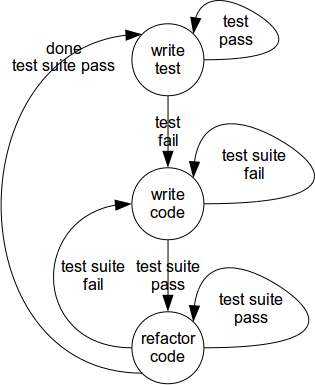
\includegraphics[scale=0.5]{diagrams/TDD_classic}
    \caption{TDD development cycle.}
    \label{fig:tdd_diagram}
  \end{minipage}
  \hspace{0.02\linewidth}
  \begin{minipage}[b]{0.48\linewidth}
    \centering
    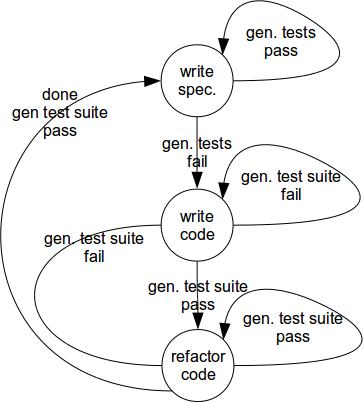
\includegraphics[scale=0.5]{diagrams/FDD_classic}
    \caption{FDD classic development cycle.}
    \label{fig:fdd_diagram}
  \end{minipage}
\end{figure}

% composition is not enough
FDD is used for the formal specified parts of the system, whether TDD is used for the remaining ones: a ``composition'' of formal and agile verification practices.
Yet there are several problems that still need to be addressed.
No communication between the two worlds is permitted, it is not defined how to formally specify a module after it has been implemented and verified in a non formal way.
A module only partially specified is a sort of hybrid that must be treated accordingly.
Finally, in the FDD cycle shown in Figure \ref{fig:fdd_diagram}, the implicit assumption is that it is always possible to identify the correct formal specifications of the system, but this is not always straighforward.
Identifying the correct formal specification is a difficult task, it has to be supported and verified by the development process.

% FDD with handmade tests
A partially specified module cannot be verified properly only through automatically generated tests.
Handmade tests have to be used together with generated ones.
Handmade tests verify complex behaviours that are informally specified, or complex behaviours that are formally specified but cannot be replicated by the formal verification tools, because of the limits of the verification tools themselves. 
The constraints imposed by formal verification tools~\cite{Glass2002} must be taken into account when deciding whether supporting the code with handmade tests, and verification tools based on automatically generated tests are not an exception.
The development cycle able to blend formal specifications, handmade tests and code development is shown in Figure \ref{fig:fdd_hand_made_tests_diagram}: the formal specification drives the handmade tests. 
Both handmade tests and the formal specification drive the code development.

\begin{figure}[ht]
  \begin{minipage}[b]{0.48\linewidth}
    \centering
    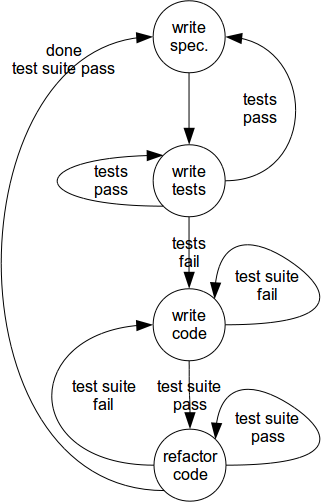
\includegraphics[scale=0.5]{diagrams/FDD_hand_made_tests}
    \caption{FDD development cycle with handmade tests.}
    \label{fig:fdd_hand_made_tests_diagram}
  \end{minipage}
  \hspace{0.02\linewidth}
  \begin{minipage}[b]{0.48\linewidth}
    \centering
    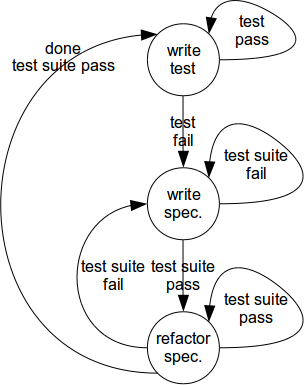
\includegraphics[scale=0.5]{diagrams/TDF}
    \caption{TDF development cycle.}
    \label{fig:tdf_diagram}
  \end{minipage}
\end{figure}

% test driven formal specification
The opposite path still needs to be covered, moving incrementally from a tested code to a formally specified code.
In this case, new handmade tests and existing working code drives the formal specification, this is what we call Test Driven Formal specification (TDF).
The resulting development cycle code is shown in Figure \ref{fig:tdf_diagram}, TDF is used to incrementally add formal specifications to an existing working system.

% all together blends into a mole
When the ``Mole'' verification practices are used together the initial objectives are achieved: an incremental and iterative process, where development pace is defined by very short development cycles similar to TDD; the complete freedom to decide what is formally specified; the development cycles and the associated verification practices maintain the corresponding artifacts involved consistent, the correct development cycle is determined by the formality of the artifacts involved, ranging from pure development cycles, shown in Figure \ref{fig:tdd_diagram} and \ref{fig:fdd_diagram}, to blended ones, shown in Figure \ref{fig:fdd_hand_made_tests_diagram} and \ref{fig:tdf_diagram}.



% =====================================================================
\section{``Mole'' verification practices applied}
\label{sec:a_complex_case_study}

\subsection{Data stream, protocol description and protocol specification}
\label{subsec:data_stream_and_protocol_description}

% protocol layers
The \SB protocol is asynchronous and packet-based; the packets have a fixed length.  
The protocol is separated in multiple layers to ease its implementation in the driver.
The layers identified are the following: (1) packet byte structure: the internal representation of the packet; (2) packet info structure: the meaningful fields contained in the packets; (3) single packet rules: the content acceptable values, and how they influence each other; (4) packet sequence rules: the content acceptable values, based on values of previously received packets; (5) packet input output asynchronous rules: the content acceptable values and reaction constraints on output packets, based on previously transmitted input packets.
The first three layers are analyzed in the case study, considering only the output sensor data packet.

% packet structure
The packet byte and info structure of the output sensor data packet reflect the board capabilities and built in sensors. 
A single packet has to accommodate various types of data: fast, medium and slow data rate streams, together with metadata describing the sensors and the board state.
The internal structure of the packet is strictly fixed. 

% packet internal structure: collection of frames
A packet is internally composed by 82 frames. 
A frame accommodates data from the fast and medium data rate streams (4 fast data rate stream and 8 medium data rate stream channels) and theirs associated metadata.
%Fast, medium and slow data rates have not a common multiple; a packet, capable to accommodate outputs at different rates, in a fixed structure, relies in two forms of redundancies, for slow and medium data rates:
%\begin{itemize}
%\item Slow data rates: slow data is located at the beginning of each packet, the data is simply repeated (it is equal to the previous packet in the stream) when no new data is available.
%\item Medium data rates: the 8 medium rate channels are multiplexed together into the medium data rate data sample of each frame. The medium data rate sample channel is a piece of info extracted from the frame description (frame metadata), including the possibility to have no data at all. 
%E.g. a frame contain a medium data rate sample from channel 0, the following frame a sample from channel 5, the following frame no sample at all, etc.
%\end{itemize}

% single packet rules
The single packet rules delimit the boundaries of the values obtainable from the packet: each defined sensor represented in the packet, as well as the metadata describing the \STSB and the packet and frame contents, are constrained by a range of acceptable values.
There are also rules affecting more than one value, and rules specifying a correct sequence of frames.



%\subsection{Data stream and protocol specification}
%\label{subsec:data_stream_and_protocol_specification}

% protocol specification
The specifications of the protocol are distilled and refined incrementally.
The protocol is divided in various (thin) layers, and each of the layer is verified with a different approach: some of the layers are specified formally. 

\paragraph*{Packet byte structure specification}

% verification
Verification is obtained through an handmade test suite, composed of unit and integration tests; the tests specifies the behaviours of the implementation, which is capable of recognizing the proper packet structure in a binary data stream. 
%The implementation is tricky: it searches for repeated patterns into a byte stream to be sufficiently confident on how the stream is decomposed into packets.
The packet byte structure is not stable: the internal byte structure changed several times during development.
Therefore, packet byte structure is informally specified.

% development cycles
The test suites are used to verify board simulators (low-level), but they cannot be used to check properties at runtime.
Code and tests are implemented using TDD.

\paragraph*{Packet info structure specification}

% verification
Verification is provided by handmade test suite, JML annotations and generated unit test suite. 
It has been built starting from handmade tests only (TDD development cycles).
Later on JML annotations have been added incrementally, using a mix of ``Mole'' practices: to move from handmade tests to formal specifications, TDF have been initially used; than all the ``Mole'' practices have been used according to the artifacts involved.

% development cycles
The test suites are used to verify board simulators (high-level), RAC and JML annotations are used to check the formally specified properties at runtime.
Code and tests have been initially implemented using TDD, than using all the ``Mole'' verification practices.

\paragraph*{Single packet rules}

% verification
The verification is provided exclusively by the formal specification with JML language, combined with the generated unit test suite and handmade test suite to verify the most complex behaviour.
It is built starting from JML annotations, supported by handmade tests when needed.

% development cycles
The test suites are used to verify board simulators (high-level), RAC and JML annotations are used to check most of the rules at runtime.
Code and tests are implemented using both forms of FDD.



\paragraph*{On simulators}
%\label{subsec:on_simulators}

% why simulators are useful
Simulators are used to test parts of the system minimizing dependencies: a simulator can be used by upper layers, with no need to provide the functionalities of the lower layers. 
%The simulators proved essential during the development, since the physical board was not available. 

% simulators description
The layer structure is not matched by the corresponding simulators.
The driver API is splitted in two abstraction layers: the general high-level interface, that exposes the main functionalities of the board and the main contents of the packets, and the lower level implementation that parses the data streams in and out the board, meant to translate the higher level instructions and data in properly formed packets.
The simulators are built according to these abstraction layers.
The high-level simulator implements the interfaces providing the methods to deal with an abstracted \SB.
The low-level simulator is capable to rebuild the \SB data streams: the in and out data streams are built exactly as the sensor board is expected to parse or generate.



\subsection{JML specification examples}
\label{subsec:a_jml_specification_example}

% a simple specification example
The JML specifications are of varying complexities.  
Some of them are rather simple, focusing on constraints that should hold when calling a method (the preconditions) and constraints on the return value (the very basic form of postconditions). 
In listing \ref{lst:jml_example_simple} a simple JML specification example is shown, the method \lil{getTemperature} is declared \lil{/*@ pure @*/}, which means that it cannot change the state of any object (a postcondition); the specification also constraints the return value with a lower and upper bound (another postcondition).

\begin{lstlisting}[
  caption={A simple specification with JML annotation: simple postconditions.},
  label=lst:jml_example_simple,
  float=htbp]
  /*@ 
      ensures \result >= -880; 
      ensures \result <= 2047; 
  @*/ 
  /*@ pure @*/ short getTemperature();
\end{lstlisting}

\sloppy

% a complex specification example
The complex specifications usually focus on properties regarding the behaviour of a whole object.
In listing \ref{lst:jml_example_invariant} a complex invariant example is shown; an invariant is a property maintained during the life cycle of an object, more precisely, an invariant is assumed on entry and guaranteed on exit of each method of an object. 
The invariant is constraining the number of samples for each medium data rate streams: the total number of streams is \lil{Frame.ADC_CHANNELS}, the total number of frames is \lil{FRAMES}, the constant constraining the number of samples is \lil{FRAMES/Frame.ADC_CHANNELS+1}, meaning that the samples contained in a frame are fairly distributed on the channels.
The valid samples are counted parsing all the frames contained in a packet, selecting only the matching valid samples.  
A medium data rate stream sample is considered valid when \lil{isADCActive()} method returns \lil{true}.

\fussy

\begin{lstlisting}[
  caption={A specification with JML annotation: a complex object invariant which constraints 
    the number of samples for each medium data rate stream channel.},
  label=lst:jml_example_invariant,
  float=htbp]
  /*@ 
      invariant ( 
        \forall int channel; 
            0 <= channel && 
            channel < Frame.ADC_CHANNELS; ( 
          \num_of int i; 
              0 <= i && 
              i < (FRAMES-1); (
            (getFrame(i).isADCActive()) && 
            (getFrame(i).getADCChannel() == channel)
          ) 
        ) <= (FRAMES / Frame.ADC_CHANNELS + 1) 
      ); 
  @*/
\end{lstlisting}



\subsection{Test cases}
\label{subsec:test_cases}

% unit tests kinds
The unit test cases that verify the protocol driver are of two kinds: handmade unit tests and automatically generated unit tests based on JML specifications; they are complementary and built to be used together.  

% unit tests effectiveness
The test effectiveness is evaluated for each test suite; the evaluation is carried out in section \ref{subsec:test_cases_retrospectives}.
The test effectiveness evaluation considers three elements: effective results on piloting the real board (quantitative), code coverage
(quantitative), development help and usefulness (qualitative).

\paragraph*{Handmade tests}

% the driver package structure
The package structure of the driver is shown in Figure \ref{fig:class_diagram_main}: two independent packages are defined (\lil{Stream} and \lil{Driver}).  
The packages are abstract, that is, they mainly contain abstractions; in Java language this is translated into a package which contains mainly abstract classes or interfaces.  
The dependency between the two abstract packages is not direct, it is realized through an implementation (\lil{StreamDriver}).
This is needed to maintain a high decoupling of the packages, and is the result of applying the dependency inversion principle~\cite{Martin1996}.

\begin{figure}[htb!]
  \centering
  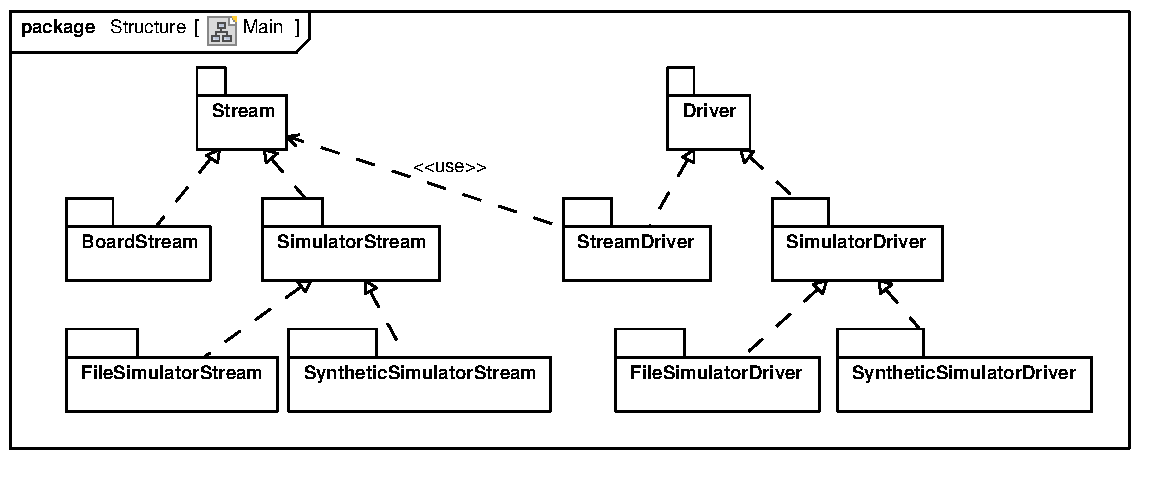
\includegraphics[scale=0.7]{UML_model/Class_Diagram__Structure__Main}
  \caption{Main packages class diagram.}
  \label{fig:class_diagram_main}
\end{figure}

% the test package structure
The test package structure, shown in Figure \ref{fig:class_diagram_test}, reflects and mimics the code structure; the tests for an abstract package are abstract, and implemented by the package that tests a corresponding system implementation. 
This is a well known test pattern (the Abstract Test Pattern~\cite{Thomas2004}) used to test that the contracts defined in the abstractions are respected in all the implementations.  
For instance, package \lil{DriverT} contains abstract tests for the abstractions of package \lil{Driver}, package \lil{StreamDriverT} inherits the abstractions of \lil{DriverT} and makes them concrete, to test the corresponding implementation \lil{StreamDriver}; package \lil{StreamDriverT} also contains stand alone tests written specifically for the implementation \lil{StreamDriver}.

\begin{figure}[htb!]
  \centering
  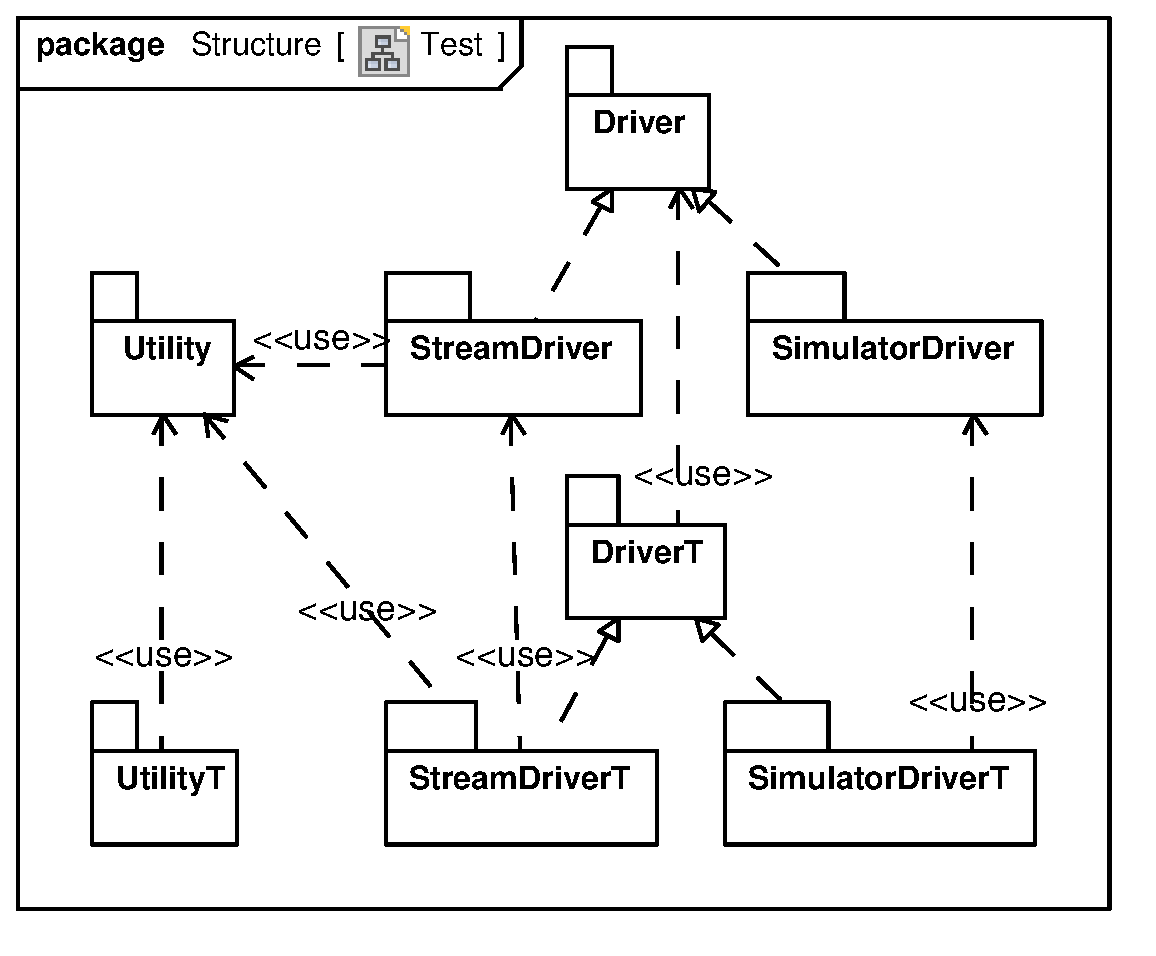
\includegraphics[scale=0.4]{UML_model/Class_Diagram__Structure__Test}
  \caption{Test packages class diagram.}
  \label{fig:class_diagram_test}
\end{figure}

\paragraph*{Generated tests}

% the generated test package structure
The JML specifications are used to generate tests.
The resulting test package structure is closely related and reflects the overall package structure; each package have a corresponding generated test package.

%\begin{figure}[htb!]
%  \centering
%  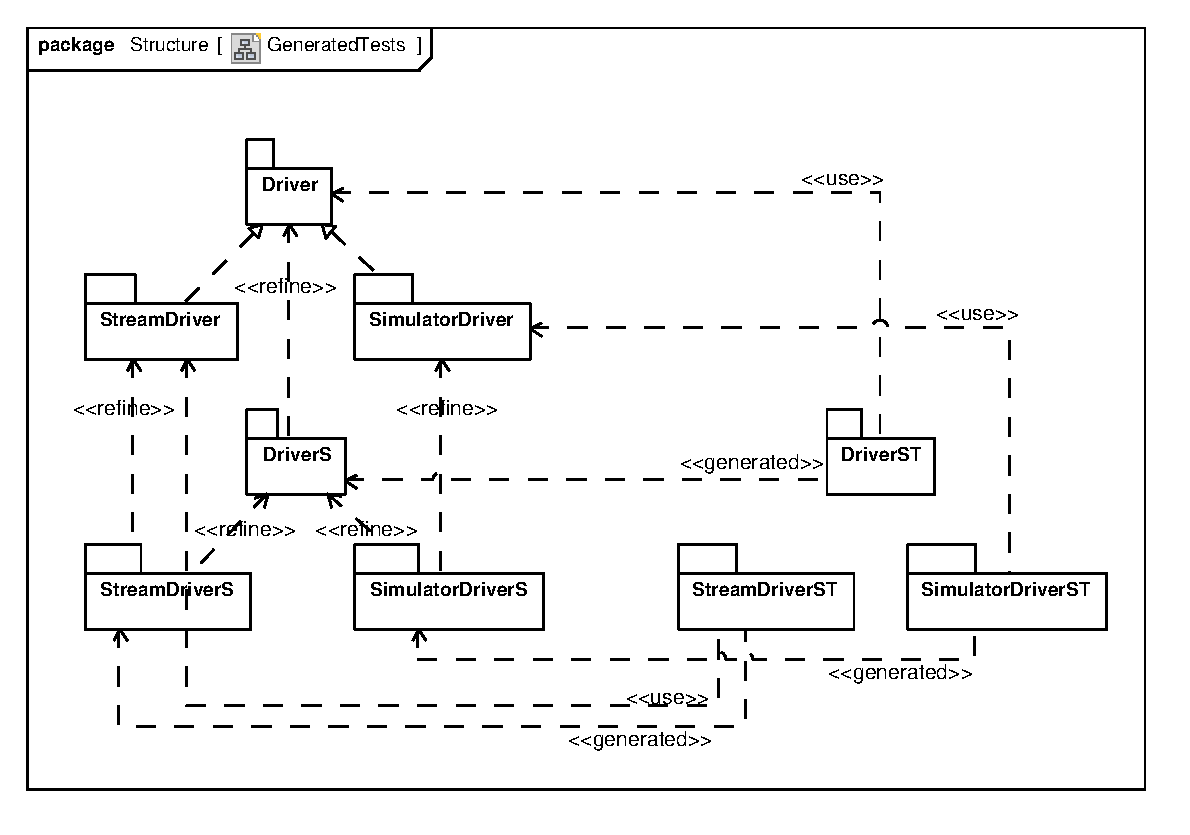
\includegraphics[scale=0.7]{UML_model/Class_Diagram__Structure__GeneratedTests}
%  \caption{Generated test packages class diagram.}
%  \label{fig:class_diagram_generatedtest}
%\end{figure}

\paragraph*{On simulators}

% simulator roles in tests
Simulators are adopted in the handmade test suits as stubs.
The resulting structure is shown in Figure \ref{fig:class_diagram_streamdriver_test}.  
For instance, in Figure \ref{fig:class_diagram_streamdriver_test} the test suite \lil{StreamDriverT} is using the \lil{SimulatorStream} to properly simulate the \lil{Stream} parsed by \lil{StreamDriver}, which is the system under test.

\begin{figure}[htb!]
  \centering
  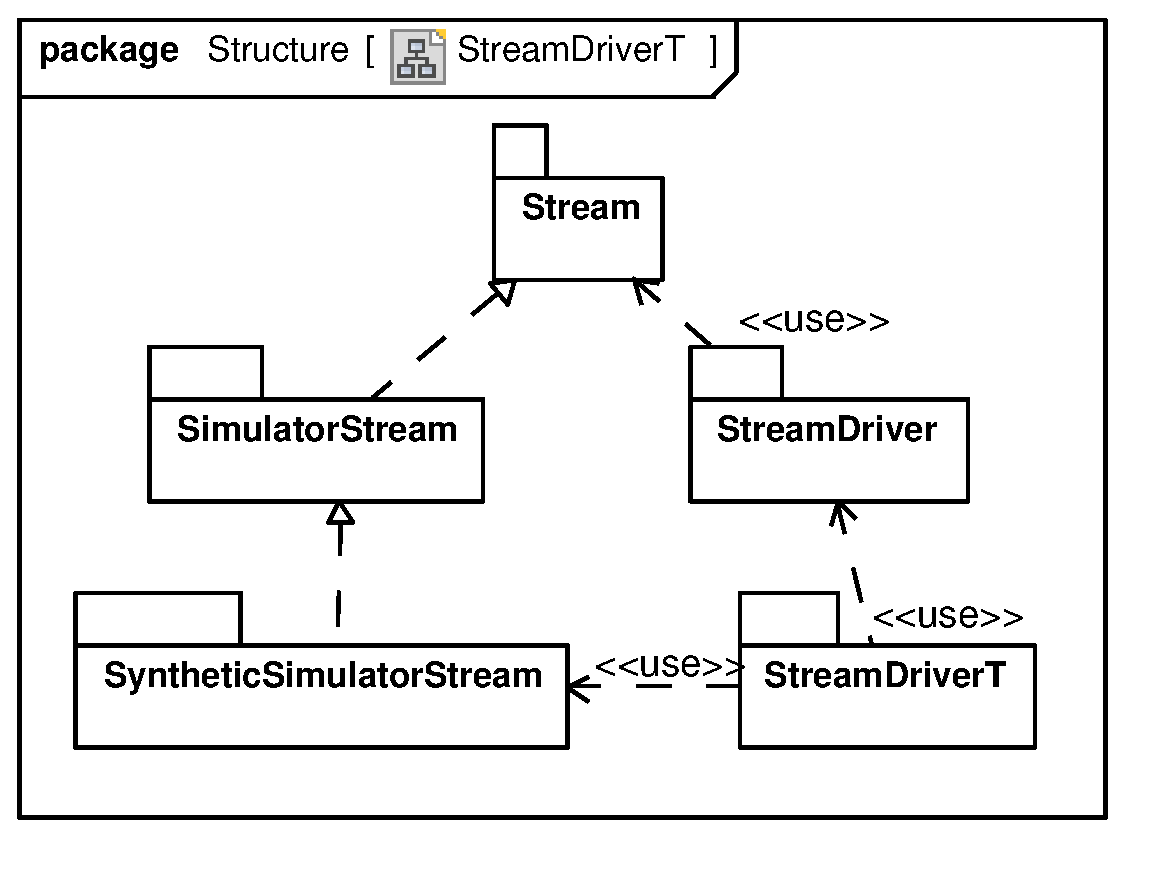
\includegraphics[scale=0.4]{UML_model/Class_Diagram__Structure__StreamDriverT}
  \caption{StreamDriver test packages class diagram: use of the stream
    simulator.}
  \label{fig:class_diagram_streamdriver_test}
\end{figure}

% simulator adoption
The simulators are adopted in both the handmade and the generated test suite; both the suites need a proper set of stubs in order to be executed.



\subsection{Test cases on the job}
\label{subsec:test_cases_on_the_job}

% test suites sizes
The handmade test suite is composed by over 140 tests, while the generated one is 100 times bigger, totalling over 14000 tests.
The large number of generated tests are explained looking closely at how the generated tests are created by the JML framework. 
The generated tests explore the possible input combinations on public methods, combining the type data ranges that are specified for the test suite (see \cite{Cheon-Leavens02} for more details on how the JML framework works on generating unit tests). 
For instance, let's suppose a method \lil{m(int p1, int p2)} must be tested in a class \lil{C}; the data ranges specified for type \lil{int} are \lil{\{1,2,3\}} and for type \lil{C} are the instances \lil{\{c1,c2,c3,c4\}}. 
The JML framework generates $24 = 3 \times 3 \times 4$ tests, since they are the combination of the data ranges involved (the data range of the parameters and the data range of the type owning the method under test). 
Nevertheless, not all the generated tests are executed: a generated test is not executed, unless the preconditions of the called method are satisfied. 
Thus, depending on the preconditions specified for a method, the number of the generated tests that are actually executed in the test suite are significantly smaller compared to the total number of generated tests.

% test execution time, values
Test suites execution time are different: the handmade test suite, with the runtime assertion checking active, runs completely in less than one minute on an average PC, while the generated test suite runs in more than 20 minutes (the rough ratio is $ 1 : 60 $). 
Most of the time is spent on setting up the suite; only considering the real execution of the tests, with no suite setup, the execution time reduces to less than 4 minutes (the rough ratio is $ 1 : 10 $).

% test effectiveness
Code coverage metrics (white-box testing) are used to compare in a quantitative way the effectiveness of the test suites. 
This is only an indicator, since it is accepted that code coverage alone cannot asses the quality of a test suite\cite{Marick1999,Chockler2006}.
Various coverage metrics exist, the test suites are analyzed with statement code coverage (one of the simplest types)\footnote{The tool used to obtain statement code coverage metrics is \myhref{http://emma.sourceforge.net/}{Emma}.}: statement coverage reports whether each statement is encountered during execution. 
The coverage results are reported in the Table \ref{tab:statement_code_coverage}.

\begin{table}[htbp]
  \caption{Statement code coverage result, categorized by source package.}
  \label{tab:statement_code_coverage}
  \begin{center}
    \begin{tabular}{|c|c|c|c|}\hline
      & \textbf{\textit{hand}} & \textbf{\textit{generated}} &
      \textbf{\textit{total}} \\\hline
      \textbf{\textit{Driver}} & $15.9 \%$ & $6.3 \%$ & $15.9 \%$ \\\hline
      \textbf{\textit{StreamDriver}} & $76 \%$ & $79.7 \%$ & $88.5 \%$ \\\hline
      \textbf{\textit{SimulatorDriver}} & $64.9 \%$ & $44.2 \%$ &
      $71.2 \%$ \\\hline
      \textbf{\textit{Utility}} & $98.1 \%$ & $74.5 \%$ & $98.1 \%$ \\\hline
    \end{tabular}
  \end{center}
\end{table}



%\subsection{Retrospective on test cases effectiveness}
%\label{subsec:test_cases_retrospectives}

% <100 coverage measures, utility methods
The coverage measures reported in Table \ref{tab:statement_code_coverage} do not reach 100\%. 
This is because of the effects of both non public utility methods, and abstract methods in interfaces.
The effect of non public methods (package Java visibility) is that these methods are taken into account as public and protected ones are, during code coverage calculation; these methods are not part of the interface, the system does not depend on them, they are only used in object initialization or in object setups performed during unit tests. 
%In fact there are package and private code blocks that are not reachable by construction from public and protected methods, and this is a precise characteristic reflecting the code architecture, meant to ease class instances setup and configuration for testing purposes (white box testing). 
%The used statement coverage tool is not able to distinguish these code blocks, so this effect is unavoidable. 
The effect is mainly seen in low \lil{SimulatorDriver} code coverage figures: the \lil{SimulatorDriver} package has many utility non public methods.

% <100 coverage measures, interfaces
Regarding interfaces, an interface contains no statements, so when an interface method is called, it is the method of the implementation class used that is actually covered.
This effect is visible in \lil{Driver} coverage figures: \lil{Driver} package contains interfaces (that are not counted at all) and some very simple real class (exceptions) that are not thoroughly tested. 
%The net result is extremely low statement code coverage figures because the very simple classes are the only ones that are actually covered. 

% code coverage interpretation
The statement code coverage figures show that the test suites do a good job on the most important package, the \lil{StreamDriver}. 
The generated test suite reaches almost $ 80 \% $, while the handmade tests have only a slightly lower coverage ratio: $ 76 \% $. 
The combination of test suites raise the coverage ratio to $ 88.5 \% $. 
This is a clear indication that one test suite is not completely overlapping the other: the intuition that test suites are not alternatives, but have to be used together to achieve the higher benefits, is confirmed.
A similar indication is provided by \lil{SimulatorDriver} package as well.

% handmade unit test vs generated unit test
The qualitative difference of the two test suites are understood observing how the suites are built. 
An handmade unit test usually requires objects initialization, one or more method calls to the modules under test, and the following assertions to verify the expected state change on the modules involved. 
A generated unit test has a more focused and limited scope: only one method call is performed in each test, therefore it is difficult to explore complex behaviours. 
%Theoretically with a complete specification, and specifying large enough data ranges, the generated tests achieve the same expressive power as the handmade ones; but the specification is not complete, and a large enough data ranges is long to develop.
The test suites give their best when used in a combined approach: the generated test suite, checking simpler and formalized behaviours, and the handmade, checking the more complex ones, whether formalized or not.  



\paragraph*{Effectiveness on board delivery}

% tests and the first prototype, board side
The first \STSB prototype builds packets with no data, but the packets are built in a way not consistent with the specification.  
The board errors are detected by using the driver implementation, the \lil{StreamDriver} package.

% tests and the second prototype, driver side
The second prototype builds packets with values taken from real sensors installed on the board.  
The only sensors that are not working are the sensors devoted to the fast rate data streams (audio sensors).  
One error needed to be corrected in the driver implementation, because of a (rare) combinations of conditions not initially covered by the test cases, but that occasionally showed up during real use.
%One error was discovered in the low-level system driver used by the developed driver (the system driver is outside our development scope): to eliminate the error, an upgrade of the low-level driver to a new beta version was necessary. 
%No other errors were detected on the driver side.

% tests and the second prototype, board side
The second prototype respected the packet byte structure specification, but was not fully compliant to the packet info structure specification and the single packet rules.
It also randomly generated completely invalid packets when overheated.
The formal JML specifications and the runtime assertion checker correctly identified these errors.
4 protocol errors regarding the packet info structure specification, and 2 protocol errors regarding the single packet rules were found, as well as the invalid packets. 



\section{Retrospective on ''Mole`` practices effectiveness}
\label{subsec:test_cases_retrospectives}

% preconditions on projects
''Mole`` practices are very easy to be applied and work with.
Many projects could benefit from the practices, not only the unstable ones that requires a certain level of formality.
Even projects with no formal specification requirements at all could benefit from the practices, since some system properties are easy to specify and could actually reduce the test suites development effort.

% precondition on formal methodology and associated formal suite
The cornerstone of the practices is the FM with its supporting tools, and the precondition on the tools are not easy to be fulfilled.
Methodology that require a complete formalization are impossibile to be applied.
Beside, it is not clear if a tool suite that does not provide a run time verification environment could be used succesfully, not it is clear whether formal methods not based on the contract paradigma (preconditions and postconditions) could be applied at all.
These are open questions that will nedd to be addressed in future works to assess the real appliability of the ''Mole`` practices.

% when to use what
There no strict rules to determine which of the ''Mole`` practices to use to face a specific problem, but only advices.
TDD if we don't need anu specification, FDD with generated tests if the specification are not too difficult and the scenario is simple enough to be covered by generated tests, FDD with hand made tests if the scenarios is complex, TDF when the specification is complex.
The experience gathered is yet not enogh to distill idioms or patterns.

% what is working and what is not
FDD with hand made tests is amazing, it is as natural to work with as TDD. 
FDD with generated tests can be annoying because of the time needed to run the test suite, often only part of the test suite is executed so that the development loops take not too long.
TDF is great with complex preconditions, but really difficult with postconditions, especially if the soecification is made on top of already existing code. 
When developing postconditions after code, the test is not expected to fail, hence the feedback is limited and the specification could not be as strict as it was needed. 
In this specific case TDF effectiveness is limited.



\section{Conclusions}
\label{sec:conclusions}

% the problem
In this paper we focus on a specific set of development problems that neither agile methodologies nor FMs are completely confortable to cope with.
The problems we are interested in are characterized by unstable requirements and artifacts which must be formally specified and verified, and are constrained by deadlines that cannot be postponed.
We propose a blend of agile and formal engineering practices, enclosed by an iterative and incremental development process: the ``Mole'' development process.

% Mole
The verification practices proposed recreate the fast feedback development environment we find in Test Driven Development, used with formal and informal artifacts.
A total of four practices are presented, two of them are conservative, following closely the development practices of FMs and AMs, while the other pair are innovative, blending together elements from both worlds.

% Mole at work
The practices have been applied succesfully to develop a driver for a custom embedded sensor board, equipped with board simulators and protocol verifiers. 
The protocol and the board specifications were informal and unstable. 
Yet a working software product was needed as soon as possible, with incrementally added functionality, and keeping it linked with the last specifications of the protocol and the board.
``Mole'' verification practices enabled us to keep in sync formal specifications (JML annotations), informal specifications (test suites) and source code, through very fast and short development cycles.
We developed handmade test suites, generated test suites and JML annotations, wich succesfully supported the verification of the driver and the simulators, and the board as well, when it was delivered.

% extending Mole
The practices are very general, and are applicable to different development languages and FMs.
One important constraint is on the FM, that must be able to cope with partial specifications; another constraint is on the tools available, that must be able to verify the system properties at runtime and partially automate the verification process of the formalized properties.

%\bibliographystyle{lni}

\bibliography{extra,abbrev,ads,category,complexity,hypertext,icsr,knowledge,languages,linguistics,meta,metrics,misc,modeling,modeltheory,reuse,rewriting,softeng,specification,ssr,technology,theory,web,upcoming,upcoming_conferences,conferences,workshops,verification,escjava,jml,nijmegen}

\end{document}

